% !TEX root = ../main.tex

\todo[inline, caption = {Synthesis time as a function to number of actions ?}]{Provide data on how computationally costly/cheap behavior synthesis is. Time vs number of actions?}

Team ViGIR did not employ high-level behavior synthesis during the DRC Finals.
However, we later carried out experimental demonstrations on \textsc{Atlas} in the lab.
Due to a hardware issue, \textsc{Atlas} could not locomote.
Thus, in addition to two experimental demonstrations, we present a simulation run carried out in Gazebo, using the same operator and onboard software.
We summarize these demonstrations below.
Please also refer to the accompanying video.

\subsection{Behavior Development using Synthesis}\label{S:SynthesisFromScratch}

In the first experimental demo, we show how a high-level behavior is specified and synthesized starting from scratch\footnote{The \textsc{ltl} specification and the synthesized automaton are available at: \scriptsize{\url{https://gist.github.com/spmaniato/c37fb12e874c73d986da}}}.
Once the state machine has been instantiated (Fig. \ref{Fig:stand_and_pick_sm}), it is ready for execution (Fig. \ref{Fig:stand_and_pick_gopro}).

\begin{figure}[t]
	\centering
	\begin{subfigure}[b]{0.99\columnwidth}
	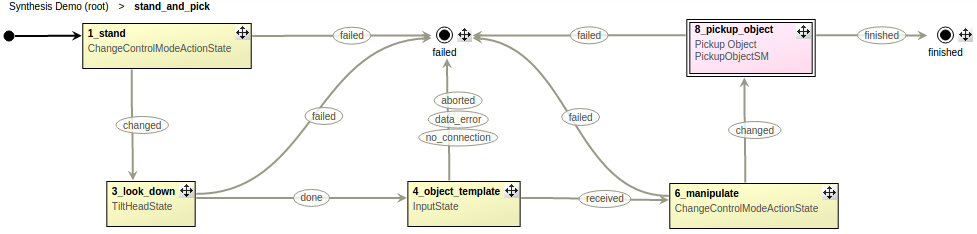
\includegraphics[width=0.99\columnwidth,clip]{./img/stand_and_pick_sm.png}
	\caption{
	The state machine above was synthesized for the task with $\mathcal{I} = \{ \mathtt{stand\_prep} \}$ and $\mathcal{G} = \{ \mathtt{look\_down}, \mathtt{pickup\_object} \}$.
	The capability $\mathtt{object\_template}$ requests an object template from the operator (Section \ref{S:TeamViGIR}).
	It is a precondition of $\mathtt{pickup\_object}$.
	}
	\label{Fig:stand_and_pick_sm}
	\end{subfigure}
	
	\vspace{4 pt}
	\begin{subfigure}[b]{0.95\columnwidth}
	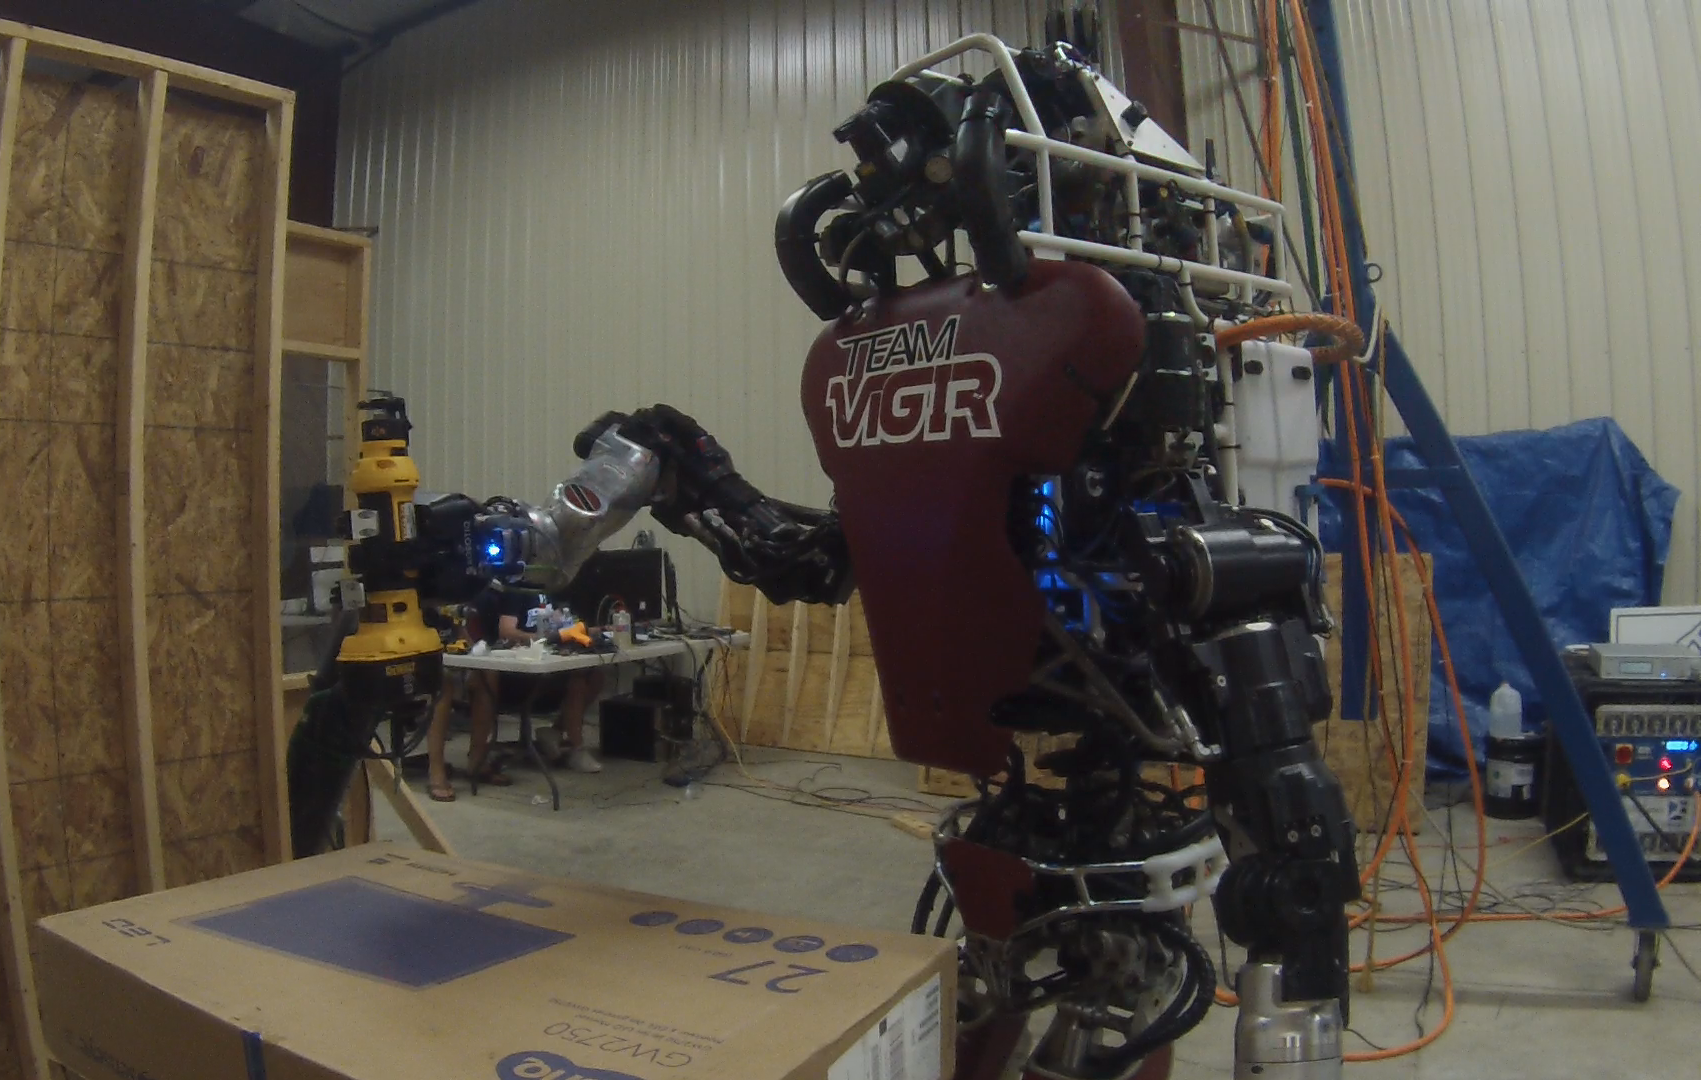
\includegraphics[width=0.99\columnwidth, clip]{./img/stand_and_pick_gopro.png}
	\caption{\textsc{Atlas} finishing execution of state $\mathtt{8\_pickup\_object}$.
	} 
	\label{Fig:stand_and_pick_gopro}
	\end{subfigure}
	\caption{
	Snapshots from the demo in Section \ref{S:SynthesisFromScratch}.
	}
	\label{Fig:stand_and_pick_demo}
\end{figure}

\subsection{Online Modifications using Synthesis}\label{S:RuntimeSynthesis}

For the second experimental demonstration, consider a scenario where the operator has designed a state machine that addresses a high-level task (either manually or via synthesis).
\textsc{Atlas} is then deployed and starts carrying out this task.
If, during execution, an \emph{unexpected} situation arises, the operator can use FlexBE's runtime modification capability (Fig. \ref{Fig:synthesis_runtime_demo}).
In this case, behavior execution is ``locked" (paused) at some state (Fig. \ref{Fig:runtime1}) and the operator specifies a new high-level behavior meant to address the unexpected situation.
Once this new state machine is instantiated (Fig. \ref{Fig:runtime2}), it is connected to the previous one (Fig. \ref{Fig:runtime1}), and execution resumes.

\begin{figure}[t]
	\centering
	\begin{subfigure}[b]{0.99\columnwidth}
	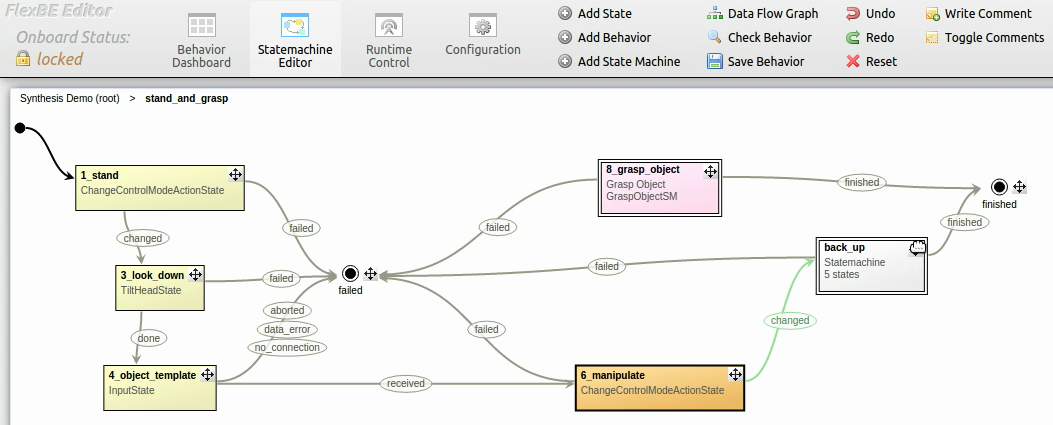
\includegraphics[width=0.99\columnwidth, clip]{./img/synthesis_runtime_connect_sm.png}
	\caption{The operator ``locks" the initial state machine at the state $\mathtt{6\_manipulate}$ (indicated by the orange color), which is allowed to be executed.
	Then, a new state machine, $\mathtt{back\_up}$, is synthesized with $\mathtt{manipulate}$ as the initial condition.
	The transition from $\mathtt{6\_manipulate}$ is then moved from $\mathtt{8\_grasp\_object}$ to $\mathtt{back\_up}$.
	} 
	\label{Fig:runtime1}
	\end{subfigure}
	
	\vspace{4 pt}
	\begin{subfigure}[b]{0.99\columnwidth}
	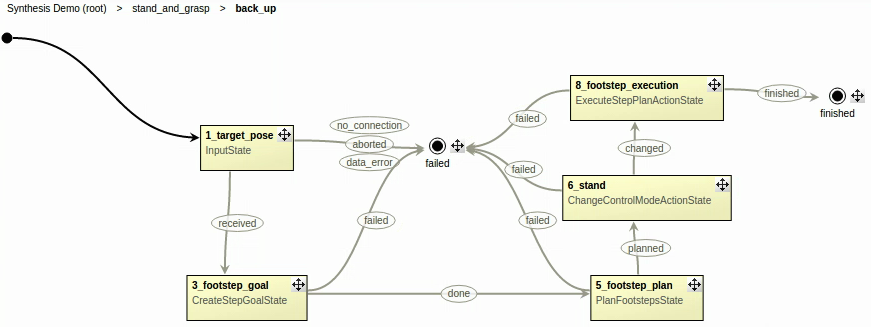
\includegraphics[width=0.99\columnwidth, clip]{./img/synthesis_runtime_synthesized_sm.png}
	\caption{The new state machine, $\mathtt{back\_up}$, was synthesized for the task with $\mathcal{I} = \{ \mathtt{manipulate} \}$ and $\mathcal{G} = \{ \mathtt{footstep\_execution} \}$.
	} 
	\label{Fig:runtime2}
	\end{subfigure}
	\caption{
	FlexBE Editor snapshots from the demo in Section \ref{S:RuntimeSynthesis}.
%	During execution of the $\mathtt{stand\_and\_grasp}$ state machine, an unexpected situation arises.
	In response to some unexpected event, the operator synthesized a state machine that has \textsc{Atlas} back away (\ref{Fig:runtime2}).
	}
	\label{Fig:synthesis_runtime_demo}
\end{figure}

%\subsection{Infinite execution or Footstep stuff (simulation)}
%
%For example, ``From stand-prep, walk to object, pick it up, (go to stand-manipulate), carry object, release, and repeat"

% END